% Please keep this introductory single-source illustration separate from the
% later packed-screen / peeling figure; it adds no new algorithmic step.
\begin{figure}[!t]
\centering
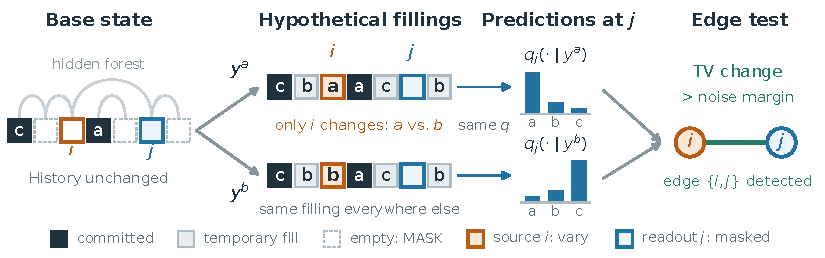
\includegraphics[width=\linewidth]{figures/intro_counterfactual_2026-09-20/output/pdf/intro_counterfactual_2026-09-20.pdf}
\caption{Counterfactual edge probing; faint arcs show the hidden forest.
 Keeping the committed state unchanged,
 vary only source $i$ between two hypothetical fillings and compare the
 predicted rows at masked readout $j$. With the same fully filled background,
 a response above the oracle-noise margin detects $\{i,j\}$.
 Section~\ref{sec:main-packed-screen} packs and aggregates such tests.}
\label{fig:intro-counterfactual-20260920}
\end{figure}
